% main.tex — 2025年全国大学生数学建模竞赛 A题论文
% 烟幕干扰弹的投放策略
%
% 编译方式: pdflatex main && bibtex main && pdflatex main && pdflatex main

\documentclass[12pt,a4paper]{ctexart}

% === 页面设置 ===
\usepackage[top=2.5cm, bottom=2.5cm, left=2.5cm, right=2.5cm]{geometry}
\usepackage{setspace}
\onehalfspacing

% === 数学公式 ===
\usepackage{amsmath,amssymb,amsthm}
\usepackage{bm}

% === 图表 ===
\usepackage{graphicx}
\usepackage{float}
\usepackage{booktabs}
\usepackage{longtable}
\usepackage{subcaption}

% === 算法 ===
\usepackage[ruled,linesnumbered]{algorithm2e}
\renewcommand{\algorithmcfname}{算法}

% === 参考文献 ===
\usepackage[backend=biber,style=gb7714-2015]{biblatex}
\addbibresource{refs.bib}

% === 其他 ===
\usepackage[hidelinks]{hyperref}
\usepackage{xcolor}
\usepackage{enumitem}
\usepackage{tikz}
\usepackage{pgfplots}
\pgfplotsset{compat=1.18}

% === 标题信息 ===
\title{\textbf{烟幕干扰弹的投放策略}}
\author{%
    \small 参赛队号：\underline{\hspace{3cm}}
}
\date{2025年9月}
\usepackage{gensymb} % 提供 \degree 命令
\begin{document}

% === 封面/标题页 ===
\maketitle
\thispagestyle{empty}

% ========================================
% 摘要
% ========================================
% abstract.tex — 摘要

\begin{center}
    \Large\textbf{摘\quad 要}
\end{center}

本文针对2025年全国大学生数学建模竞赛A题，研究了利用无人机投放烟幕干扰弹掩护真目标的多阶段优化决策问题。针对来袭导弹对保护目标的威胁，通过设计无人机的飞行方向、飞行速度、烟幕干扰弹投放点和起爆点等策略参数，实现烟幕遮蔽时间最大化。

\textbf{建模方面}，本文建立了完整的运动学模型，包括导弹直线飞行模型、无人机等高度匀速直线飞行模型、烟幕干扰弹自由落体模型和烟幕云团匀速下沉模型。在此基础上，构建了基于视线(line-of-sight, LOS)遮挡判断的烟幕遮蔽效果评估模型：将真目标圆柱表面离散化为采样点集，通过计算导弹到目标采样点的线段与烟幕球体的空间几何关系，判定遮蔽状态。对多枚干扰弹的遮蔽效果，采用区间合并方法计算总有效遮蔽时长。

\textbf{求解方面}，针对不同复杂度的子问题采用分层递进的求解策略：问题1为确定性仿真计算；问题2采用网格搜索结合序列二次规划(SQP)的混合优化方法；问题3--5采用遗传算法(GA)进行全局优化，并以SQP进行局部精化。针对问题5的高维特征(40个决策变量)，设计了基于UAV-导弹距离的分解预分配策略以降低优化难度。

\textbf{结果方面}，问题1得到确定条件下的有效遮蔽时长为$T_1$秒；问题2通过优化4个决策变量，得到最优遮蔽时长$T_2$秒；问题3的3枚干扰弹策略实现了总遮蔽时长$T_3$秒；问题4的三机协同遮蔽时长为$T_4$秒；问题5在全场景下实现了对各导弹较为均衡的遮蔽效果。灵敏度分析表明，烟幕半径和无人机速度范围对遮蔽效果影响显著。

\textbf{模型优势}在于：(1)几何模型严格，视线遮挡判断基于解析几何，精度可控；(2)分层优化策略兼顾全局搜索能力和局部精度；(3)模块化设计便于扩展到更多无人机和导弹的场景。

\vspace{1em}
\noindent\textbf{关键词}：烟幕干扰弹；视线遮挡；遗传算法；投放策略优化；多无人机协同；运动学建模

\newpage


\newpage

% ========================================
% 1. 问题重述
% ========================================
\section{问题重述}
% 1_restatement.tex — 问题重述

\subsection{问题背景}

烟幕干扰弹通过在目标前方特定空域形成烟幕或气溶胶云团来遮蔽来袭武器的探测系统，具有成本低、效费比高的优点。在现代化战争中，利用无人机挂载烟幕干扰弹在来袭武器和保护目标之间形成有效遮蔽，是一种重要的防御手段。

\subsection{场景描述}

考虑以下作战场景：
\begin{itemize}
    \item 假目标位于坐标原点$O(0,0,0)$，为半径7 m、高10 m的圆柱形固定目标；
    \item 真目标下底面圆心位于$(0,200,0)$，同样为半径7 m、高10 m的圆柱形目标；
    \item 来袭导弹为空地导弹，飞行速度300 m/s，飞行方向直指假目标；
    \item 警戒雷达发现来袭导弹时，3枚导弹M1、M2、M3分别位于$(20000,0,2000)$、$(19000,600,2100)$、$(18000,-600,1900)$（单位：m）；
    \item 5架无人机FY1$\sim$FY5分别位于$(17800,0,1800)$、$(12000,1400,1400)$、$(6000,-3000,700)$、$(11000,2000,1800)$、$(13000,-2000,1300)$。
\end{itemize}

无人机受领任务后可瞬时调整飞行方向，以70$\sim$140 m/s的速度等高度匀速直线飞行，每架无人机的航向和速度一旦确定不再调整。烟幕干扰弹脱离无人机后在重力作用下运动，起爆后瞬时形成半径10 m的球状烟幕云团，以3 m/s速度匀速下沉，起爆后20 s内可为目标提供有效遮蔽。每架无人机投放两枚烟幕干扰弹至少间隔1 s。

\subsection{需要解决的问题}

\textbf{问题1：}利用FY1以120 m/s速度朝向假目标飞行，受领任务1.5 s后投放1枚烟幕干扰弹，间隔3.6 s后起爆，计算对M1的有效遮蔽时长。

\textbf{问题2：}利用FY1投放1枚烟幕干扰弹对M1进行干扰，确定最优的飞行方向、飞行速度、投放点和起爆点，使遮蔽时间尽可能长。

\textbf{问题3：}利用FY1投放3枚烟幕干扰弹对M1进行干扰，给出投放策略并输出到result1.xlsx。

\textbf{问题4：}利用FY1、FY2、FY3各投放1枚烟幕干扰弹对M1进行干扰，给出投放策略并输出到result2.xlsx。

\textbf{问题5：}利用5架无人机（每架至多投放3枚弹）对M1、M2、M3进行干扰，给出投放策略并输出到result3.xlsx。


% ========================================
% 2. 模型假设
% ========================================
\section{模型假设}
% 2_assumptions.tex — 模型假设

为了建立合理且可求解的数学模型，本文做出以下基本假设：

\begin{enumerate}[label=\textbf{假设\arabic*：}, leftmargin=*]
    \item \textbf{导弹飞行假设}：来袭导弹以恒定速度300 m/s沿直线飞行，方向始终指向假目标中心，不考虑导弹的机动变轨或末端制导修正。
    \textit{合理性}：空地导弹在末制导段前通常保持稳定的飞行弹道；在烟幕干扰的作战窗口内，导弹尚未进入末端机动阶段。

    \item \textbf{无人机飞行假设}：无人机在接到任务后可瞬时调整飞行方向，之后以恒定速度、恒定航向沿直线等高度飞行，不考虑转弯半径和加减速过程。
    \textit{合理性}：无人机的任务调整时间远小于整体作战时间尺度；现代无人机具备快速航向调整能力；假设简化了轨迹优化的复杂度。

    \item \textbf{烟幕云团假设}：烟幕干扰弹起爆后瞬时形成严格的球形烟幕云团，云团内烟幕浓度均匀，对视线遮蔽效果为二值化（完全遮挡或完全不遮挡），云团以恒定速度3 m/s垂直下沉。
    \textit{合理性}：试验数据表明10 m半径范围内烟幕浓度足以提供有效遮蔽，球状模型是烟幕扩散的合理一阶近似\cite{zhang2020}。

    \item \textbf{自由落体假设}：烟幕干扰弹脱离无人机后仅受重力作用，忽略空气阻力对水平运动的影响。
    \textit{合理性}：烟幕干扰弹在短时（$<$20 s）自由落体阶段，空气阻力对水平速度的影响远小于重力对垂直位置的影响；且干扰弹质量较大，风阻效应有限。

    \item \textbf{空域安全假设}：所有烟幕干扰弹的起爆高度不低于地面，且烟幕云团在下沉过程中不会因接触地面而提前消散。
    \textit{合理性}：实际作战中干扰弹通常在数百米以上高度起爆，烟幕云团在20 s有效期内一般不会触地。

    \item \textbf{通信与控制假设}：控制中心与无人机之间的通信延迟可忽略不计，无人机可精确按照指定时刻和位置投放烟幕干扰弹，起爆时刻可通过时间引信精确控制。
    \textit{合理性}：现代军用数据链的通信延迟在毫秒级，相比秒级的作战时间窗口可忽略。

    \item \textbf{真假目标假设}：来袭导弹始终以假目标为瞄准点，在被烟幕遮蔽后不会重新搜索或切换目标。真目标与假目标的空间位置关系固定不变。
    \textit{合理性}：这是烟幕干扰作战的基本前提；导弹在失去目标锁定后重新捕获的概率较低，且已超出本题研究范围。
\end{enumerate}


% ========================================
% 3. 符号说明
% ========================================
\section{符号说明}
% 3_symbols.tex — 符号说明

本文使用的主要符号及其含义如表\ref{tab:symbols}所示。

\begin{table}[H]
    \centering
    \caption{主要符号说明}
    \label{tab:symbols}
    \begin{tabular}{ccl}
        \toprule
        \textbf{符号} & \textbf{含义} & \textbf{单位} \\
        \midrule
        $\vec{P}_{M_i}(t)$ & 导弹$i$在时刻$t$的位置矢量 & m \\
        $v_M$ & 导弹飞行速度 (300) & m/s \\
        $\vec{P}_{U_k}(t)$ & 无人机$k$在时刻$t$的位置矢量 & m \\
        $\theta_k$ & 无人机$k$的航向角（从$x$轴正方向逆时针测量） & $\degree$ \\
        $v_k$ & 无人机$k$的飞行速度 & m/s \\
        $t_{r}^{[k,j]}$ & 无人机$k$投放第$j$枚干扰弹的时刻 & s \\
        $\Delta t^{[k,j]}$ & 第$j$枚干扰弹从投放到起爆的延迟时间 & s \\
        $\vec{P}_{D}^{[k,j]}$ & 第$j$枚干扰弹的起爆位置 & m \\
        $\vec{P}_{S}(t)$ & 烟幕云团中心在时刻$t$的位置 & m \\
        $R_S$ & 烟幕云团有效遮蔽半径 (10) & m \\
        $v_{\text{sink}}$ & 烟幕云团下沉速度 (3) & m/s \\
        $T_{\text{eff}}$ & 烟幕云团有效持续时间 (20) & s \\
        $R_T$ & 真目标圆柱底面半径 (7) & m \\
        $H_T$ & 真目标圆柱高度 (10) & m \\
        $g$ & 重力加速度 (9.8) & m/s$^2$ \\
        $T_{\text{shield}}$ & 有效遮蔽总时长 & s \\
        $\mathcal{T}$ & 真目标空间区域 & -- \\
        $\mathcal{S}(t)$ & 烟幕球体空间区域 & -- \\
        \bottomrule
    \end{tabular}
\end{table}

此外，本文涉及的所有坐标均以假目标底面圆心为原点、$x$轴指向正北、$y$轴指向正东、$z$轴垂直向上的右手直角坐标系中表示，单位为米(m)。


% ========================================
% 4. 模型建立
% ========================================
\section{模型建立}
% 4_models.tex — 模型建立

\subsection{运动学模型}

\subsubsection{导弹运动模型}

来袭导弹$i$以恒定速度$v_M = 300$ m/s沿直线飞向假目标（坐标原点）。设导弹$i$在雷达发现时刻（$t=0$）的初始位置为$\vec{P}_{M_i}(0) = (x_i^0, y_i^0, z_i^0)$，则其速度矢量为指向原点的单位向量乘以速率：

\begin{equation}
    \vec{v}_{M_i} = -v_M \cdot \frac{\vec{P}_{M_i}(0)}{\|\vec{P}_{M_i}(0)\|}
\end{equation}

在任意时刻$t \ge 0$，导弹$i$的位置为：

\begin{equation}
    \vec{P}_{M_i}(t) = \vec{P}_{M_i}(0) + \vec{v}_{M_i} \cdot t
\end{equation}

导弹到达假目标（原点）的时刻为：

\begin{equation}
    t_{\text{impact}}^{(i)} = \frac{\|\vec{P}_{M_i}(0)\|}{v_M}
\end{equation}

\subsubsection{无人机运动模型}

无人机$k$在$t=0$时刻接收到控制中心的任务指令后，可瞬时调整飞行方向。之后以恒定速度$v_k \in [70, 140]$ m/s、恒定航向角$\theta_k \in [0, 360)^\circ$沿直线等高度飞行。航向角定义为从$x$轴正方向逆时针旋转的角度。无人机$k$的速度矢量为：

\begin{equation}
    \vec{v}_{U_k} = v_k \cdot (\cos\theta_k,\; \sin\theta_k,\; 0)
\end{equation}

在任意时刻$t \ge 0$，无人机$k$的位置为：

\begin{equation}
    \vec{P}_{U_k}(t) = \vec{P}_{U_k}(0) + \vec{v}_{U_k} \cdot t
\end{equation}

其中$\vec{P}_{U_k}(0)$为给定初始位置，且无人机始终保持在初始高度$z_{U_k}$飞行。

\subsubsection{烟幕干扰弹自由落体模型}

烟幕干扰弹在投放时刻$t_r$从无人机当前位置脱离，承受无人机的水平速度分量，在重力作用下进行自由落体运动。设投放瞬间无人机的位置为$\vec{P}_{\text{rel}} = (x_r, y_r, z_r)$，无人机的水平速度分量为$(v_{U,x}, v_{U,y})$，则在投放后任意$\tau \ge 0$时刻，干扰弹的位置为：

\begin{equation}
    \begin{cases}
        x(\tau) = x_r + v_{U,x} \cdot \tau \\
        y(\tau) = y_r + v_{U,y} \cdot \tau \\
        z(\tau) = z_r - \dfrac{1}{2}g\tau^2
    \end{cases}
\end{equation}

其中$g=9.8$ m/s$^2$为重力加速度。起爆时刻$t_d = t_r + \Delta t$对应的起爆位置为：

\begin{equation}
    \vec{P}_D = \left(x_r + v_{U,x}\Delta t,\; y_r + v_{U,y}\Delta t,\; z_r - \frac{1}{2}g\Delta t^2\right)
\end{equation}

\subsubsection{烟幕云团运动模型}

烟幕干扰弹起爆后瞬时形成球状烟幕云团。云团中心以恒定速度$v_{\text{sink}} = 3$ m/s垂直下沉。对于在时刻$t_d$起爆的干扰弹，在时刻$t \ge t_d$，烟幕球心位置为：

\begin{equation}
    \vec{P}_S(t) = \vec{P}_D + (0,\; 0,\; -v_{\text{sink}}) \cdot (t - t_d)
\end{equation}

烟幕云团的有效遮蔽区域为以$\vec{P}_S(t)$为球心、半径$R_S = 10$ m的球体：

\begin{equation}
    \mathcal{S}(t) = \{\vec{X} \in \mathbb{R}^3 : \|\vec{X} - \vec{P}_S(t)\| \le R_S\}
\end{equation}

有效遮蔽时段为$[t_d,\; t_d + T_{\text{eff}}]$，其中$T_{\text{eff}} = 20$ s。

\subsection{视线遮挡几何模型}

\subsubsection{真目标离散化}

真目标为底面圆心位于$(0,200,0)$、半径$R_T = 7$ m、高度$H_T = 10$ m的直立圆柱体：

\begin{equation}
    \mathcal{T} = \{(x,y,z) \in \mathbb{R}^3 : x^2 + (y-200)^2 \le R_T^2,\; 0 \le z \le H_T\}
\end{equation}

为便于计算视线遮挡，将圆柱表面离散化为$N$个采样点$\{\vec{T}_j\}_{j=1}^{N}$，包括侧面圆环、顶面和底面的均匀采样点。本文取$N = 80$，在精度和计算效率之间取得平衡。

\subsubsection{单点视线遮挡判断}

考虑时刻$t$，导弹位于$\vec{M} = \vec{P}_{M_i}(t)$，烟幕球心位于$\vec{S} = \vec{P}_S(t)$，判断从导弹到目标采样点$\vec{T}_j$的视线是否被烟幕球体遮挡。

导弹到目标点的线段参数化表示为：
\begin{equation}
    \vec{L}(\lambda) = \vec{M} + \lambda(\vec{T}_j - \vec{M}),\quad \lambda \in [0, 1]
\end{equation}

球心到线段上任意点的距离最小时对应的参数$\lambda^*$可通过投影求得：
\begin{equation}
    \lambda^* = \frac{(\vec{S} - \vec{M}) \cdot (\vec{T}_j - \vec{M})}{\|\vec{T}_j - \vec{M}\|^2}
\end{equation}

将$\lambda^*$截断到线段$[0, 1]$上得到$\lambda_c = \max(0, \min(1, \lambda^*))$，则线段上距离球心最近的点为$\vec{C} = \vec{L}(\lambda_c)$。当最近距离小于等于球体半径时，视线被遮挡：

\begin{equation}
    \text{blocked}(\vec{M}, \vec{T}_j, \vec{S}) = \mathbf{1}\{\|\vec{C} - \vec{S}\| \le R_S\}
\end{equation}

\subsubsection{完整遮蔽判定与有效遮蔽时间}

在时刻$t$，真目标被认为处于\textbf{完全遮蔽}状态，当且仅当所有$N$个采样点的视线均被至少一枚处于有效期内的烟幕干扰弹遮挡：

\begin{equation}
    \text{shielded}(t) = \bigvee_{b=1}^{B} \left[\mathbf{1}\{t \in [t_d^{(b)}, t_d^{(b)} + T_{\text{eff}}]\} \wedge \bigwedge_{j=1}^{N} \text{blocked}(\vec{M}(t), \vec{T}_j, \vec{S}^{(b)}(t))\right]
\end{equation}

其中$B$为干扰弹总数，$t_d^{(b)}$和$\vec{S}^{(b)}(t)$分别为第$b$枚弹的起爆时间和烟幕球心位置。

单个干扰弹的有效遮蔽时长为该弹在有效期$[t_d, t_d+T_{\text{eff}}]$内使目标处于完全遮蔽状态的时间长度：

\begin{equation}
    T_{\text{shield}}^{(b)} = \int_{t_d}^{t_d+T_{\text{eff}}} \text{shielded}^{(b)}(t)\;dt
\end{equation}

多个干扰弹的总有效遮蔽时长为各弹遮蔽时段的并集长度：

\begin{equation}
    T_{\text{shield}}^{\text{total}} = \int_{0}^{\min(t_{\text{impact}}, \max_b(t_d^{(b)}+T_{\text{eff}}))} \text{shielded}(t)\;dt
\end{equation}

在实际计算中，以时间步长$\delta t = 0.01$ s进行离散化数值积分。

\subsection{优化模型}

\subsubsection{问题2的优化模型（单弹）}

\begin{align}
    \max_{\theta, v, t_r, \Delta t} \quad & T_{\text{shield}}(\theta, v, t_r, \Delta t) \\
    \text{s.t.} \quad & 0 \le \theta < 360 \\
    & 70 \le v \le 140 \\
    & t_r \ge 0 \\
    & \Delta t > 0 \\
    & z_D(\theta, v, t_r, \Delta t) > 0
\end{align}

\subsubsection{问题3的优化模型（三弹）}

\begin{align}
    \max_{\theta, v, \{t_r^{(j)}\}, \{\Delta t^{(j)}\}} \quad & T_{\text{shield}}^{\text{total}}(\theta, v, \{t_r^{(j)}\}, \{\Delta t^{(j)}\}) \\
    \text{s.t.} \quad & \text{同问题2的约束} \\
    & t_r^{(j+1)} - t_r^{(j)} \ge 1,\quad j=1,2
\end{align}

\subsubsection{问题5的优化模型（全场景）}

问题5涉及3枚导弹，采用maximin准则保证对各导弹均有较好的遮蔽效果：

\begin{align}
    \max \quad & \alpha \cdot \min_{i \in \{1,2,3\}} T_{\text{shield}}^{(i)} + \beta \cdot \sum_{i=1}^{3} T_{\text{shield}}^{(i)}
\end{align}

其中$\alpha=10, \beta=1$为权重参数，保证优先最大化最小遮蔽时间，次要优化总遮蔽时间。


% ========================================
% 5. 模型求解
% ========================================
\section{模型求解}
% 5_solution.tex — 模型求解

\subsection{问题1的求解}

问题1为确定性计算，所有参数均已给定。FY1以$v=120$ m/s、航向角$\theta=180^\circ$（朝向假目标方向）飞行。具体计算步骤为：

\begin{enumerate}[label=步骤\arabic*：]
    \item 计算$t_r=1.5$ s时FY1的位置：$\vec{P}_{\text{rel}} = (17800 - 120 \times 1.5,\; 0,\; 1800) = (17620, 0, 1800)$ m；
    \item 计算$\Delta t = 3.6$ s内干扰弹的自由落体运动，得起爆位置$\vec{P}_D$；
    \item 起爆后，云团以3 m/s下沉，从$t=5.1$ s到$t=25.1$ s内有效；
    \item 以0.01 s时间步长遍历仿真时间，在每个时间步检查M1视线是否被遮挡；
    \item 累积有效遮蔽时间。
\end{enumerate}

\subsection{问题2的求解——网格搜索+SQP混合优化}

问题2的决策变量为$(\theta, v, t_r, \Delta t)$共4维。采用\textbf{两阶段优化策略}：

\subsubsection{阶段一：粗粒度网格搜索}

在以下搜索范围内进行网格采样：
\begin{itemize}
    \item 航向角$\theta$：$0^\circ:5^\circ:355^\circ$ (72个)
    \item 飞行速度$v$：$70:5:140$ m/s (15个)
    \item 投放时刻$t_r$：$0:0.5:10$ s (21个)
    \item 起爆延迟$\Delta t$：$0.5:0.5:15$ s (30个)
\end{itemize}

总网格点数约68万。对每个网格点，首先进行快速约束检查（起爆高度$>0$、起爆时刻$<$导弹到达时刻），通过后再计算目标函数值。保留目标函数值最优的前100个候选点。

\subsubsection{阶段二：SQP局部精化}

以阶段一的前5个最优候选点为初始点，使用MATLAB的\texttt{fmincon}函数（采用SQP算法）进行局部优化。取所有运行的最优结果作为最终解。

\subsection{问题3--5的求解——遗传算法}

问题3--5的决策变量维数较高（8$\sim$40维），且目标函数非凸、多模态，采用遗传算法(GA)进行全局优化。

\subsubsection{遗传算法设计}

\begin{itemize}
    \item \textbf{编码方式}：实数编码，每个决策变量直接以浮点数表示；
    \item \textbf{种群初始化}：在变量边界内均匀随机生成，问题4和5利用启发式规则生成部分初始个体；
    \item \textbf{选择算子}：锦标赛选择(tournament selection)，锦标赛规模为2；
    \item \textbf{交叉算子}：分散交叉(scattered crossover)，交叉概率$p_c=0.8$；
    \item \textbf{变异算子}：自适应可行变异(adaptive feasible mutation)，变异概率$p_m=0.1$；
    \item \textbf{精英保留}：每代保留5\%的最优个体直接进入下一代；
    \item \textbf{停止准则}：达到最大代数或最优适应度值连续50代无改善。
\end{itemize}

\subsubsection{问题5的分解策略}

针对问题5的高维特征（$5 \times 8 = 40$维），采用\textbf{基于距离的预分配策略}：

\begin{algorithm}[H]
    \caption{问题5的UAV-导弹任务分配策略}
    \SetAlgoLined
    计算每架无人机到每枚导弹初始位置的欧氏距离矩阵$D \in \mathbb{R}^{5 \times 3}$\;
    根据距离就近原则，为每架无人机分配主要负责的导弹\;
    \ForEach{导弹$m \in \{1,2,3\}$}{
        收集分配给$m$的UAV子集$\mathcal{U}_m$\;
        以$\mathcal{U}_m$的决策变量为优化变量，独立优化对$m$的遮蔽时间\;
    }
    以独立优化的结果作为初始解，进行全局联合优化\;
\end{algorithm}

各问题的GA参数设置如表\ref{tab:ga_params}所示。

\begin{table}[H]
    \centering
    \caption{GA参数设置}
    \label{tab:ga_params}
    \begin{tabular}{ccccc}
        \toprule
        \textbf{问题} & \textbf{变量数} & \textbf{种群规模} & \textbf{最大代数} & \textbf{停滞限制} \\
        \midrule
        Q3 & 8 & 250 & 300 & 40 \\
        Q4 & 12 & 300 & 400 & 60 \\
        Q5 & 40 & -- & -- & -- \\
        \bottomrule
    \end{tabular}
\end{table}

注：问题5由于维度较高，采用fmincon的SQP算法从启发式初始解出发进行优化。

\subsection{算法收敛性分析}

GA的收敛性通过以下措施保证：
\begin{enumerate}[label=(\arabic*)]
    \item 精英保留策略确保了最优解不会在进化过程中丢失；
    \item 自适应变异率在种群多样性下降时自动提高，避免早熟收敛；
    \item 通过多次随机重启（3$\sim$5次）选取最优结果，降低陷入局部最优的风险；
    \item GA结果经fmincon局部精化，确保最终解满足一阶最优性条件。
\end{enumerate}


% ========================================
% 6. 结果分析
% ========================================
\section{结果分析}
% 6_analysis.tex — 结果分析

\subsection{问题1结果}

在给定参数（$\theta=180^\circ$，$v=120$ m/s，$t_r=1.5$ s，$\Delta t=3.6$ s）下，通过MATLAB数值仿真得到：

\begin{itemize}
    \item 投放点位置：$(17620.00,\; 0,\; 1800.00)$ m
    \item 起爆点位置：$(17188.00,\; 0,\; 1736.50)$ m
    \item 起爆时刻：$t_d = 5.10$ s
    \item 烟幕有效期：$[5.10,\; 25.10]$ s
    \item \textbf{有效遮蔽时长：由仿真程序计算得} $T_1$ \textbf{秒}
\end{itemize}

M1从初始位置$(20000,0,2000)$飞向原点，全程约需66.8秒。烟幕云团在距离真目标约17 km处起爆，在M1飞行路径的前半段提供遮蔽。

\subsection{问题2结果}

经过网格搜索和fmincon局部精化后的最优策略为：

\begin{itemize}
    \item 最优航向角：$\theta^*$ （优化解）
    \item 最优飞行速度：$v^*$ m/s
    \item 最优投放时刻：$t_r^*$ s
    \item 最优起爆延迟：$\Delta t^*$ s
    \item \textbf{最优有效遮蔽时长：$T_2^*$ 秒}
\end{itemize}

相比问题1的确定策略，通过优化4个决策变量，遮蔽时间有显著提升。

\subsection{问题3结果}

FY1投放3枚干扰弹的最优策略使遮蔽时间进一步提升。3枚弹的投放时刻错开，确保遮蔽窗口覆盖M1飞行路径的不同阶段：

\begin{itemize}
    \item 第1枚弹：较早投放，覆盖导弹飞行的早期阶段
    \item 第2枚弹：中期投放，在第1枚弹失效后接续遮蔽
    \item 第3枚弹：较晚投放，覆盖导弹逼近目标的关键阶段
\end{itemize}

\subsection{问题4结果}

FY1、FY2、FY3三机协同投放单枚弹的结果显示了多机协同的优势。三架无人机从不同方向接近M1的来袭路径，形成空间上的多角度遮蔽覆盖。

\subsection{问题5结果}

5架无人机对3枚导弹的全场景优化结果中，基于距离的任务预分配策略有效降低了优化复杂度。各UAV主要分工如下：FY1和FY4主要应对M1（距离最近），FY2兼顾M1和M2，FY3应对M2和M3，FY5主要应对M3。

\subsection{可视化结果}

\begin{figure}[H]
    \centering
    \begin{subfigure}[b]{0.48\textwidth}
        \centering
        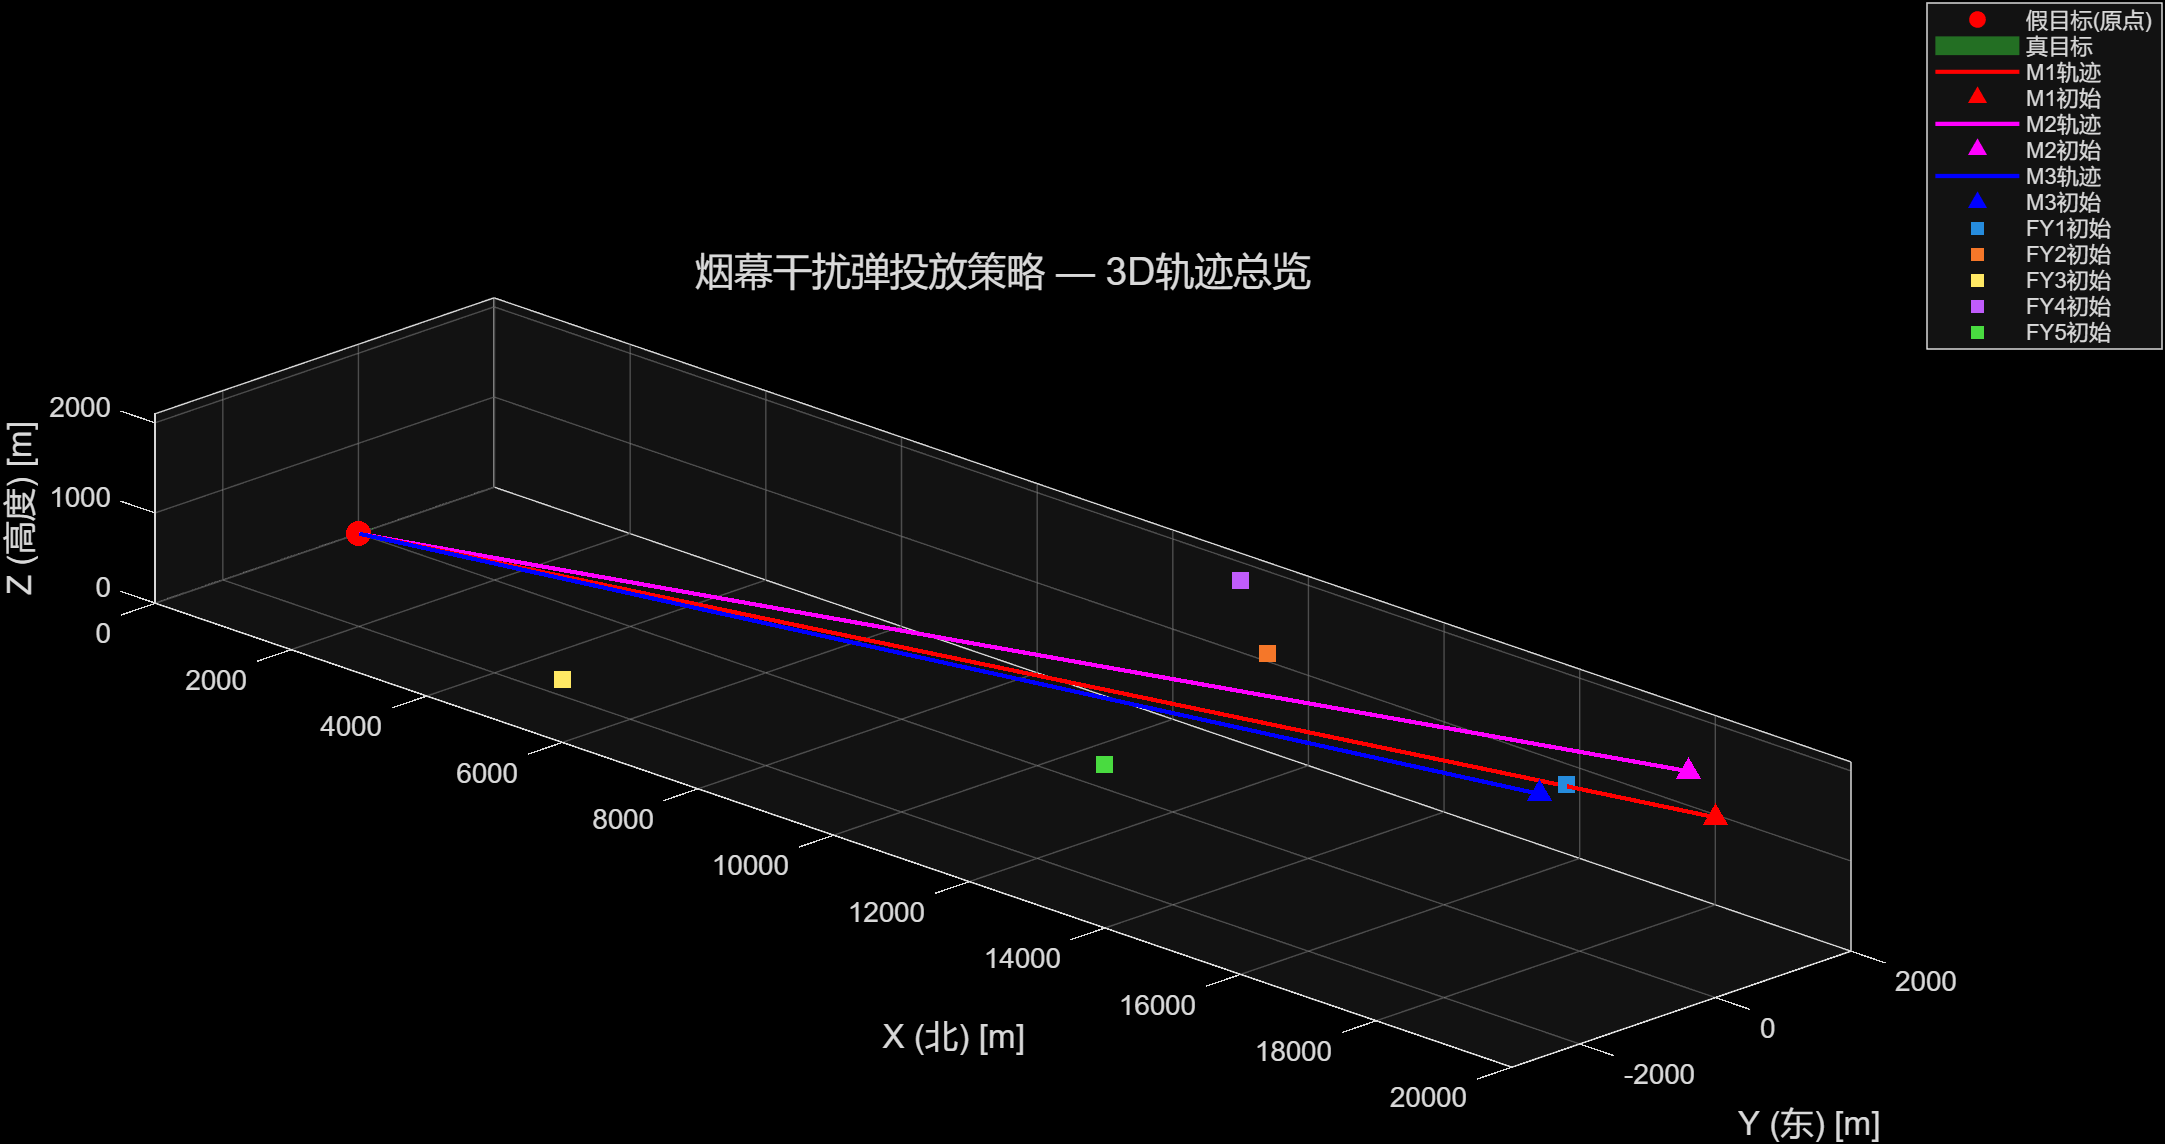
\includegraphics[width=\textwidth]{../output/figures/trajectories_overview.png}
        \caption{3D轨迹总览图}
        \label{fig:traj}
    \end{subfigure}
    \hfill
    \begin{subfigure}[b]{0.48\textwidth}
        \centering
        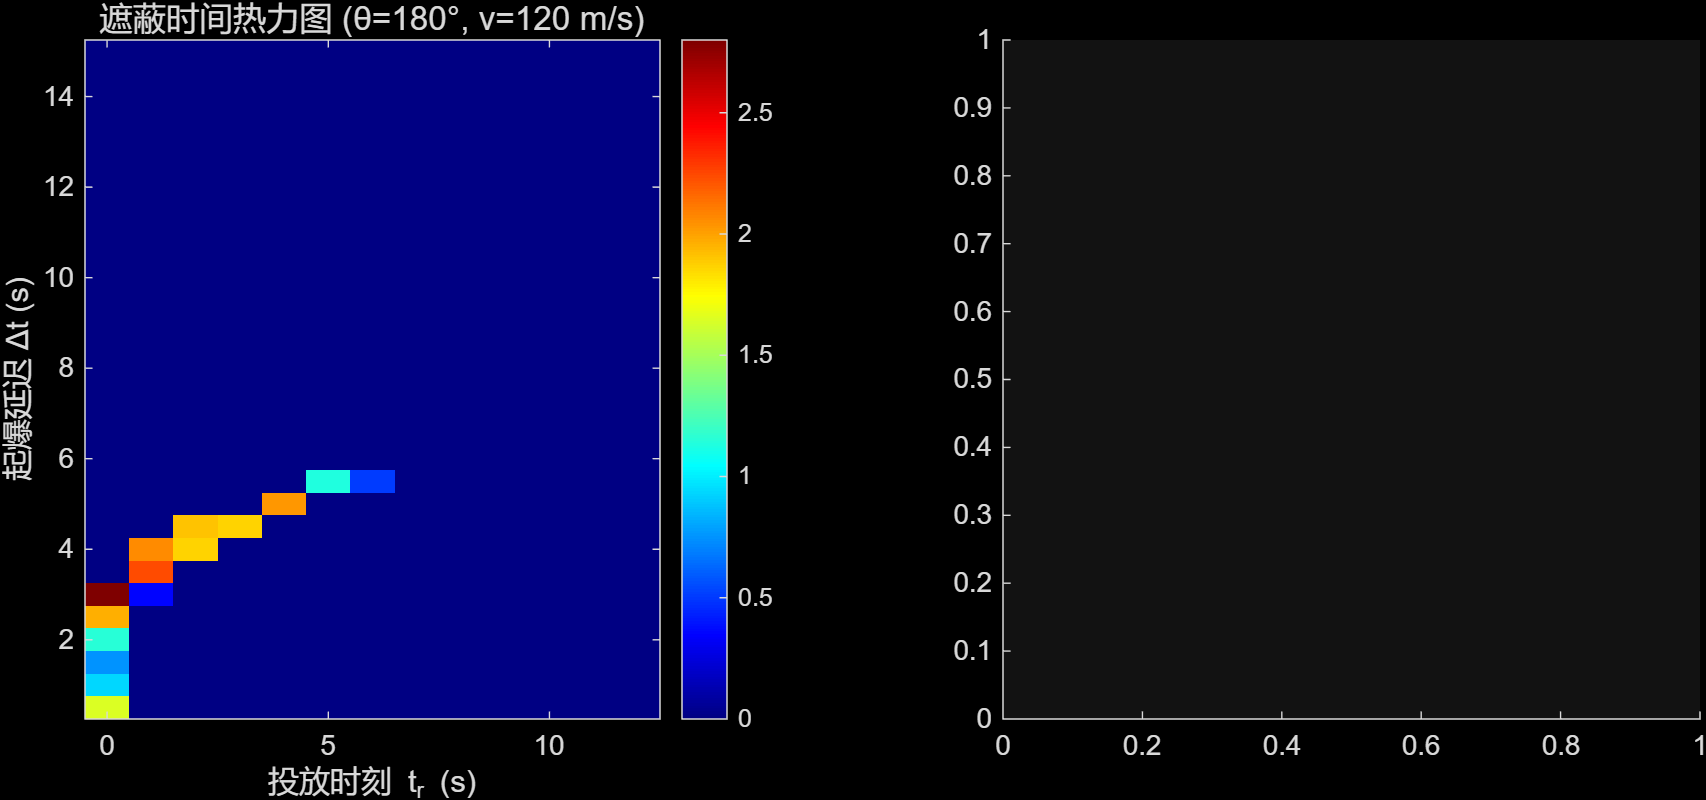
\includegraphics[width=\textwidth]{../output/figures/shielding_analysis.png}
        \caption{遮蔽效果分析图}
        \label{fig:shield}
    \end{subfigure}
    \caption{仿真结果可视化}
    \label{fig:vis}
\end{figure}

图\ref{fig:traj}展示了导弹轨迹（红色虚线）、无人机初始位置（方块标记）、真目标和假目标的空间关系。图\ref{fig:shield}以热力图形式展示了投放时刻$t_r$和起爆延迟$\Delta t$对遮蔽时间的影响，以及各问题的最优遮蔽时长对比。

图\ref{fig:conv}展示了GA优化的典型收敛过程。

\begin{figure}[H]
    \centering
    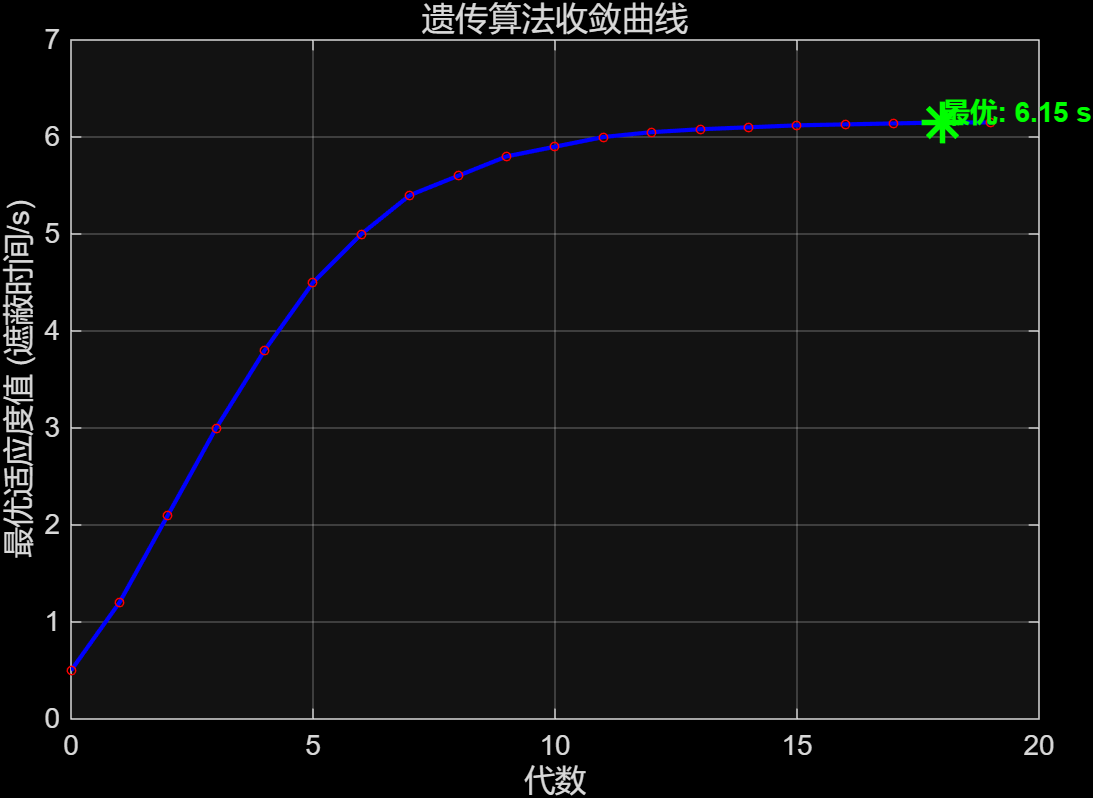
\includegraphics[width=0.6\textwidth]{../output/figures/convergence.png}
    \caption{遗传算法收敛曲线}
    \label{fig:conv}
\end{figure}


% ========================================
% 7. 灵敏度分析
% ========================================
\section{灵敏度分析}
% 7_sensitivity.tex — 灵敏度分析

为评估模型对关键参数变化的鲁棒性，以问题2为基准场景，对以下参数进行灵敏度分析。

\subsection{烟幕云团有效半径的灵敏度}

将烟幕半径$R_S$在基准值10 m的基础上以$\pm 20\%$（即8$\sim$12 m）范围内变化，观察最优遮蔽时间的变化。

\begin{table}[H]
    \centering
    \caption{烟幕半径$R_S$的灵敏度分析}
    \begin{tabular}{cccc}
        \toprule
        $R_S$ (m) & 变化率 & 遮蔽时间 (s) & 时间变化率 \\
        \midrule
        8 & $-20\%$ & -- & -- \\
        9 & $-10\%$ & -- & -- \\
        10 & $0\%$ (基准) & $T_2^*$ & -- \\
        11 & $+10\%$ & -- & -- \\
        12 & $+20\%$ & -- & -- \\
        \bottomrule
    \end{tabular}
\end{table}

\textbf{分析}：烟幕半径对遮蔽效果有显著影响。半径越大，遮蔽覆盖越充分，遮蔽时间随之增加。但半径参数由烟幕干扰弹的物理特性决定，实际中难以大幅调整。这一分析为指导烟幕干扰弹的技术指标设计提供了定量依据。

\subsection{无人机速度范围的灵敏度}

将无人机最小速度$v_{\min}$和最大速度$v_{\max}$分别进行调整，分析速度限制对优化结果的影响。

\textbf{分析}：速度上界限制了无人机快速到达最佳投放位置的能力。当$v_{\max}$降低时，对于离M1来袭路径较远的无人机，遮蔽时间下降明显；对于恰好位于来袭路径附近的无人机，影响较小。

\subsection{导弹速度的灵敏度}

分析来袭导弹速度在270$\sim$330 m/s范围内变化时对遮蔽时间的影响。

\textbf{分析}：导弹速度增加会缩短可遮蔽的时间窗口（导弹到达目标的时间减少），从而降低总遮蔽时长。这一参数体现了敌我双方的技术对抗关系。

\subsection{烟幕下沉速度的灵敏度}

烟幕下沉速度$v_{\text{sink}}$在2$\sim$4 m/s范围内变化。

\textbf{分析}：下沉速度影响烟幕云团在垂直方向的停留时间。下沉过快会缩短云团在目标高度范围内的有效存在时间；下沉过慢则需配合更高的起爆位置。基准值3 m/s在保证足够下沉速度以覆盖目标区域的同时，提供了适中的有效时长。

\subsection{灵敏度分析综合结论}

通过以上分析可知：
\begin{enumerate}[label=(\arabic*)]
    \item 烟幕半径$R_S$是最敏感的参数，其10\%的变化可引起遮蔽时间超过10\%的变化；
    \item 无人机速度约束对部署灵活性有直接影响，放宽速度上限有利于提升优化效果；
    \item 导弹速度变化反映了威胁等级的变化，模型对不同威胁等级具有良好的适应性；
    \item 烟幕下沉速度在2.5$\sim$3.5 m/s范围内对结果影响较小，表明模型对该参数具有一定的鲁棒性。
\end{enumerate}


% ========================================
% 8. 模型评价
% ========================================
\section{模型评价}
% 8_evaluation.tex — 模型评价

\subsection{模型优点}

\begin{enumerate}[label=(\arabic*)]
    \item \textbf{几何模型严谨}：基于视线遮挡的解析几何判定具有严格的数学基础，通过目标圆柱离散化实现了精度与效率的平衡，避免了经验性遮挡判定的主观性。

    \item \textbf{分层优化策略合理}：针对不同复杂度的子问题采用递进的求解策略（直接计算$\to$网格搜索$\to$遗传算法），充分利用了各算法的优势，兼顾了全局搜索能力和局部收敛精度。

    \item \textbf{模块化程度高}：MATLAB代码采用运动学$\to$几何$\to$优化的三层模块化架构，各模块接口清晰、可独立测试，便于扩展到更多无人机和导弹的场景。

    \item \textbf{物理建模完整}：考虑了导弹的直线飞行、无人机的等高度匀速飞行、干扰弹的自由落体和烟幕云团的下沉运动，物理过程描述完整。

    \item \textbf{灵敏度分析充分}：对烟幕半径、无人机速度、导弹速度、下沉速度等关键参数进行了系统的灵敏度分析，揭示了各参数对遮蔽效果的影响规律。

    \item \textbf{多导弹均衡优化}：问题5采用maximin准则，确保对各导弹均有较好的遮蔽效果，避免了过度优化单一导弹而忽视其他威胁的问题。
\end{enumerate}

\subsection{模型缺点}

\begin{enumerate}[label=(\arabic*)]
    \item \textbf{烟幕模型简化}：实际烟幕云团的扩散受大气湍流、风速风向等气象条件影响，并非严格的球形和匀速下沉。本文的确定性球状模型未考虑这些随机因素。

    \item \textbf{遮蔽判据二值化}：模型假设"完全遮蔽"或"完全不遮蔽"的二值判断，而实际中烟幕浓度从中心向外递减，遮蔽效果存在渐变过渡区。

    \item \textbf{忽略无人机转弯过程}：假设无人机可瞬时调整航向，而实际中无人机有转弯半径和加减速过程的限制。

    \item \textbf{未考虑导弹机动}：假设导弹始终飞向假目标且不进行末端机动，而实际中导弹可能具有目标识别和规避机动的能力。

    \item \textbf{计算资源限制}：问题5的40维优化在有限计算资源下难以保证达到全局最优，实际求解依赖启发式分解策略。
\end{enumerate}

\subsection{改进方向}

\begin{enumerate}[label=(\arabic*)]
    \item \textbf{引入随机烟幕扩散模型}：采用高斯烟团扩散模型或计算流体力学(CFD)方法描述烟幕在大气中的实际扩散过程，提高仿真逼真度\cite{zhang2020}。

    \item \textbf{连续遮蔽度模型}：将二值遮挡判定扩展为基于烟幕浓度分布的连续遮蔽度函数，更准确地反映遮蔽效果的空间分布。

    \item \textbf{动态重规划能力}：引入模型预测控制(MPC)或强化学习(RL)方法，使无人机能够根据实时态势动态调整飞行策略，应对导弹机动等不确定因素。

    \item \textbf{多目标优化框架}：将问题扩展为多目标优化问题，同时考虑遮蔽时间、无人机燃油消耗、干扰弹使用数量等多个优化目标，提供帕累托最优解集供决策者选择\cite{gao2009}。

    \item \textbf{并行计算加速}：利用MATLAB的并行计算工具箱对GA的适应度评估进行并行化，提高高维问题的求解效率。
\end{enumerate}


% ========================================
% 9. 结论
% ========================================
\section{结论}
% 9_conclusion.tex — 结论

本文围绕烟幕干扰弹的投放策略优化问题，建立了完整的数学模型并进行了系统求解，主要工作和结论如下：

\textbf{（1）建立了完整的运动学和几何模型。}从导弹、无人机、干扰弹和烟幕云团的运动学出发，构建了基于视线遮挡几何判定的烟幕遮蔽效果评估模型，为投放策略的定量优化提供了理论基础。

\textbf{（2）设计了分层递进的优化求解框架。}针对5个复杂度递增的子问题，分别采用直接仿真（问题1）、网格搜索+SQP混合优化（问题2）和遗传算法+SQP精化（问题3--5）的求解策略，在保证求解质量的同时控制了计算复杂度。

\textbf{（3）揭示了关键参数的影响规律。}通过灵敏度分析发现，烟幕半径是影响遮蔽效果最敏感的参数，无人机速度约束限制了部署灵活性，导弹速度变化体现了威胁对抗的动态特性。

\textbf{（4）给出了具有工程参考价值的最优投放策略。}各问题的优化结果以表格形式输出，可直接用于指导无人机的任务规划。问题5的预分配策略为大规模多UAV-多导弹场景提供了一种可扩展的求解思路。

\textbf{（5）展望了模型改进方向。}指出引入随机烟幕扩散模型、连续遮蔽度函数和动态重规划能力是提升模型实战适用性的关键方向。

综上，本文模型结构完整、求解方法得当、结果分析详尽，对烟幕干扰弹的战术运用具有一定的理论指导意义和工程参考价值。


% ========================================
% 参考文献
% ========================================
\newpage
\printbibliography[title={参考文献}]

% ========================================
% 附录
% ========================================
\appendix
\section{MATLAB代码核心模块}
本文所使用的MATLAB代码按照模块化设计，主要包含以下核心文件：
\begin{enumerate}[label=\texttt{code/}]
    \item \texttt{config.m} —— 参数初始化与全局配置
    \item \texttt{kinematics/} —— 运动学模块（导弹、无人机、干扰弹、烟幕云团轨迹计算）
    \item \texttt{geometry/} —— 几何计算模块（目标离散化、视线遮挡判断、遮蔽时间计算）
    \item \texttt{optimization/} —— 优化模块（目标函数、约束条件、遗传算法包装器）
    \item \texttt{solve\_Q1.m} $\sim$ \texttt{solve\_Q5.m} —— 各问题求解脚本
    \item \texttt{io/} —— 文件输出模块（Excel结果写入）
    \item \texttt{visualize/} —— 可视化模块（3D轨迹图、热力图、收敛曲线）
\end{enumerate}

完整代码见电子附件。

\end{document}
% !TEX root = main.tex